\chapter{Curvatura de la tierra}
\label{ap:tierraCurva}

	
	Debido a la curvatura de la tierra, el angulo con el que llega la lluvia al detector, \td{}, es diferente al utilizado para calcular la probabilidad de interacci\'on de los \nutau{} en la tierra, \te{}.
	Esta situaci\'on se esquematiza en la figura \ref{fig:curveEarthSketch}.
	
	\begin{figure}[ht!]
		\centering
		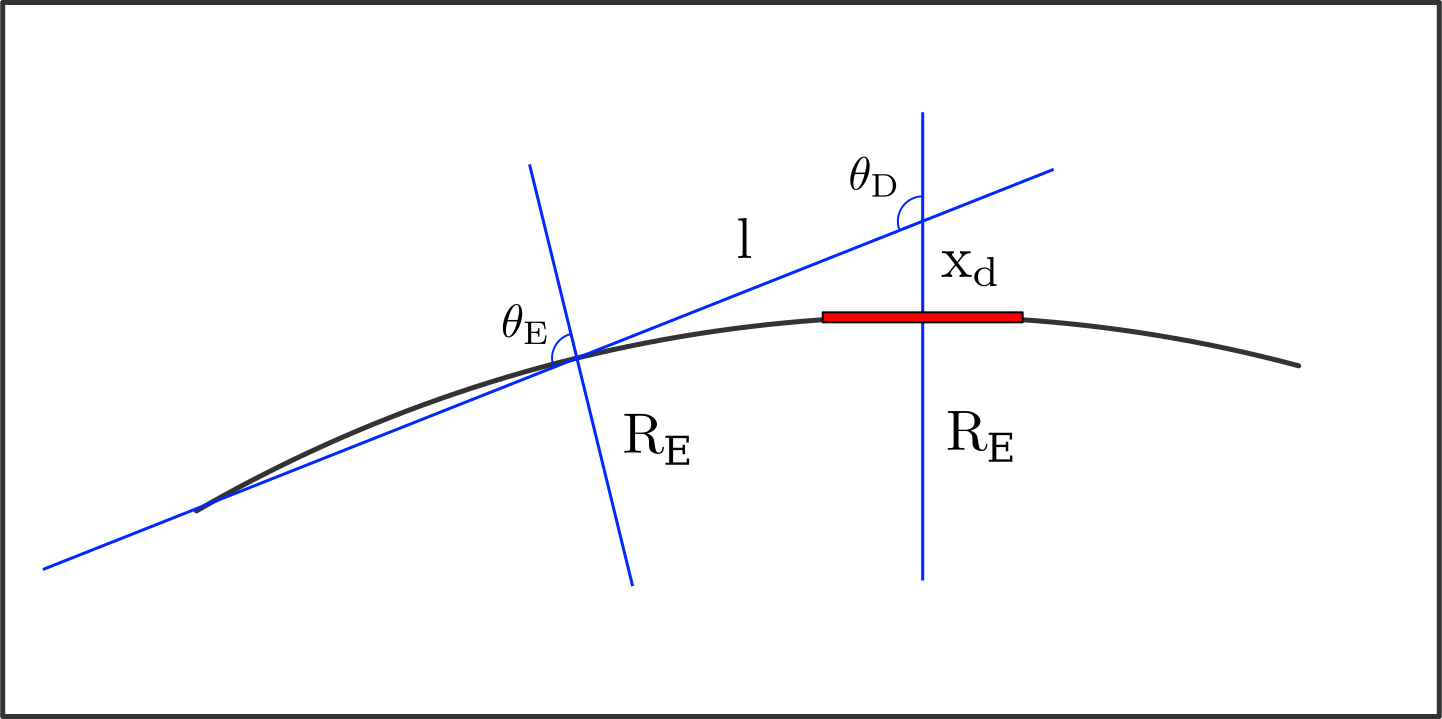
\includegraphics[width=0.8\textwidth]{./fig/appendix/curveEarthSketch.png}
		% curveEarthSketch.png: 2404x1199 pixel, 150dpi, 40.70x20.30 cm, bb=0 0 1154 575
		\caption{\label{fig:curveEarthSketch}
		Esquema del cambio en el angulo sobre el detector y el utilizado para calcular las probabilidades de interacci\'on del neutrino en la tierra.
		}
	\end{figure}
	
	Utilizando el teorema del coseno para \te{} y para el complemento de \td{} se obtiene el siguiente sistema de ecuaciones:	
	\begin{displaymath}
		\begin{array}{rcccccl}
		(R+x_d)^2 & = & l^2 & + & R^2 & - & 2 l R \cos \theta_E \\
		R^2 & = & l^2 & + & (R+x_d)^2 & + & 2 l (R+x_d) \cos \theta_D \\
		\end{array}
	\end{displaymath}
	sumando y restando se llega a:
	\begin{displaymath}
		\begin{array}{rcccl}
		0 & = & l^2 &+ & l \left[ (R+x_d) \cos \theta_D - R \cos \theta_E \right] \\
		0 & = & R^2 - (R+x_d)^2 & - & l \left[ (R+x_d) \cos \theta_D + R \cos \theta_E \right] \\
		\end{array}
	\end{displaymath}
	donde resolviendo para $l$ se obtiene la siguiente expresi\'on:
	\begin{equation}
		\begin{array}{rcl}
		l & = & \dfrac{R^2-(R+x_d)^2}{R \cos \theta_E + (R+x_d) \cos \theta_D}\\
		&&\\
		\end{array}
		\label{eq:l_curve}
	\end{equation}
	con
	\begin{equation}
		\begin{array}{rcl}
		\cos \theta_E & = & - \left[ \dfrac{R^2 - (R+x_d)^2 (1-\cos^2 \theta_D)}{R^2} \right]^{\frac{1}{2}} \\ 
		\end{array}
		\label{eq:te_td}
	\end{equation}
	
	La ecuaci\'on \ref{eq:te_td} s\'olo tiene solici\'on real si el numerador es un numero positivo, lo que ocurre si $\theta_D<\theta_D^{cut}$, donde $\theta_D^{cut}$ cumple:
	\begin{equation}
	\cos \theta_D^{cut} = \left[ \frac{2 R x_d+x_d^2}{(R+x_d)^2} \right]^{\frac{1}{2}}
	\label{eq:tdc}
	\end{equation}
	
	La interpretaci\'on de esta cantidad es sencilla si notamos que el m\'inimo \'angulo con el que los neutrinos pueden ingresar a la tierra, \te{}, es $90^\circ$. 
	Si $\theta_E=90^\circ$, el angulo con el que se observar\'a la lluvia sobre el detector ser\'a $\theta_D^{cut}$, lo que puede observarse en la figura \ref{fig:te_td}, en la que se grafica la ecuaci\'on \ref{eq:te_td} para diferentes valores de \xd{}.
	
	\begin{figure}[ht!]
		\centering
		\includegraphics[width=0.95\textwidth]{./fig/appendix/thE_thD}
		% curveEarthSketch.png: 2404x1199 pixel, 150dpi, 40.70x20.30 cm, bb=0 0 1154 575
		\caption{\label{fig:te_td}
		Gr\'afico de la ecuaci\'on \ref{eq:te_td} para diferentes valores de \xd{}.
		}
	\end{figure}
	
	Es clave notar que $\theta_D^{cut}$ depende de la altura de decaimiento del \tauon{} sobre el detector, $x_d$.
	Por ello, si se invierte la ecuaci\'on \ref{eq:tdc} es posible obtener, dado \td{}, qu\'e alturas de decaimiento \xd{} son geometricamente aceptables, lo que se muestra en la figura \ref{fig:dx_thcut}
	
	\begin{figure}[ht!]
		\centering
		\includegraphics[width=0.95\textwidth]{./fig/appendix/thetaDCut}
		% curveEarthSketch.png: 2404x1199 pixel, 150dpi, 40.70x20.30 cm, bb=0 0 1154 575
		\caption{\label{fig:dx_thcut}
		Se grafica $\rm x_d^{CUT}$ a partir de la inversi\'on de la ecuaci\'on \ref{eq:tdc}. Se observa el conjunto de par\'ametros geom\'etricamente admitidos.
		}
	\end{figure}

	Finalmente, es importante estudiar como cambia la distancia que recorre el \tauon{} en la atmosfera al tener en cuenta la curvatura de la tierra.
	Recordando la ecuaci\'on \ref{eq:l_curve} y que en la aproximaci\'on de tierra plana se utiliza la expresi\'on $l_{plano}=\frac{x_d}{\cos \theta_D}$, es posible graficar el cociente $\frac{l_{plano}}{l_{curvo}}$ para diferentes valores de \xd{} y \td{}, lo que se muestra en la figura \ref{fig:lp_lc}.
	
	\begin{figure}[ht!]
		\centering
		\includegraphics[width=0.95\textwidth]{./fig/appendix/lPlane_lCurve}
		% curveEarthSketch.png: 2404x1199 pixel, 150dpi, 40.70x20.30 cm, bb=0 0 1154 575
		\caption{\label{fig:lp_lc}
		Cociente $\frac{l_{plano}}{l_{curvo}}$ para diferentes valores de \xd{} y \td{}.
		}
	\end{figure}
